\documentclass[12pt,a4paper,twoside]{report}
	\makeatletter
	\def\@makechapterhead#1{%
  	%%%%\vspace*{50\p@}% %%% removed!
  	{\parindent \z@ \raggedright \normalfont
    	\ifnum \c@secnumdepth >\m@ne
        	\huge\bfseries \@chapapp\space \thechapter
        	\par\nobreak
        	\vskip 20\p@
    	\fi
    	\interlinepenalty\@M
    	\Huge \bfseries #1\par\nobreak
    	\vskip 40\p@
  	}}
	\def\@makeschapterhead#1{%
  	%%%%%\vspace*{50\p@}% %%% removed!
  	{\parindent \z@ \raggedright
    	\normalfont
    	\interlinepenalty\@M
    	\Huge \bfseries  #1\par\nobreak
    	\vskip 40\p@
  	}}
	\makeatother

\usepackage[utf8]{inputenc}
\usepackage[german]{babel}
\usepackage[T1]{fontenc}
\usepackage{amsmath}
\usepackage{amsfonts}
\usepackage{amssymb}
\usepackage{makeidx}
\usepackage{graphicx}
    \graphicspath{ {./images/} }
\usepackage[hidelinks]{hyperref}
	\hypersetup{
		colorlinks,
		allcolors=black
	}
\usepackage{caption}
\usepackage{subcaption}
\usepackage{pdfpages}
\usepackage{wrapfig}
\usepackage{kpfonts}
\usepackage[a4paper, width=150mm, top=25mm, bottom=25mm, bindingoffset=6mm]{geometry}
\usepackage{fancybox}
\usepackage{fancyvrb}
\usepackage{fancyhdr}
    \pagestyle{fancy}
    \fancyhead{}
    \fancyhead[RO,LE]{Kapitel \thechapter}
\usepackage{array}
\usepackage{tabularx}
\usepackage{booktabs}
\usepackage{longtable}
\usepackage{acronym}
\usepackage{csquotes}
\usepackage[backend=biber, bibencoding=utf8, style=ieee, dashed=false]{biblatex}
\addbibresource{bibliography/bib.bib}

\title{Konzeptionierung und Realisierung eines Einzelprüfstands für Buchholz- und Gasrelais}
\author{Jan Möllering}
\date{24.02.2020}


\begin{document}
\emergencystretch 3em

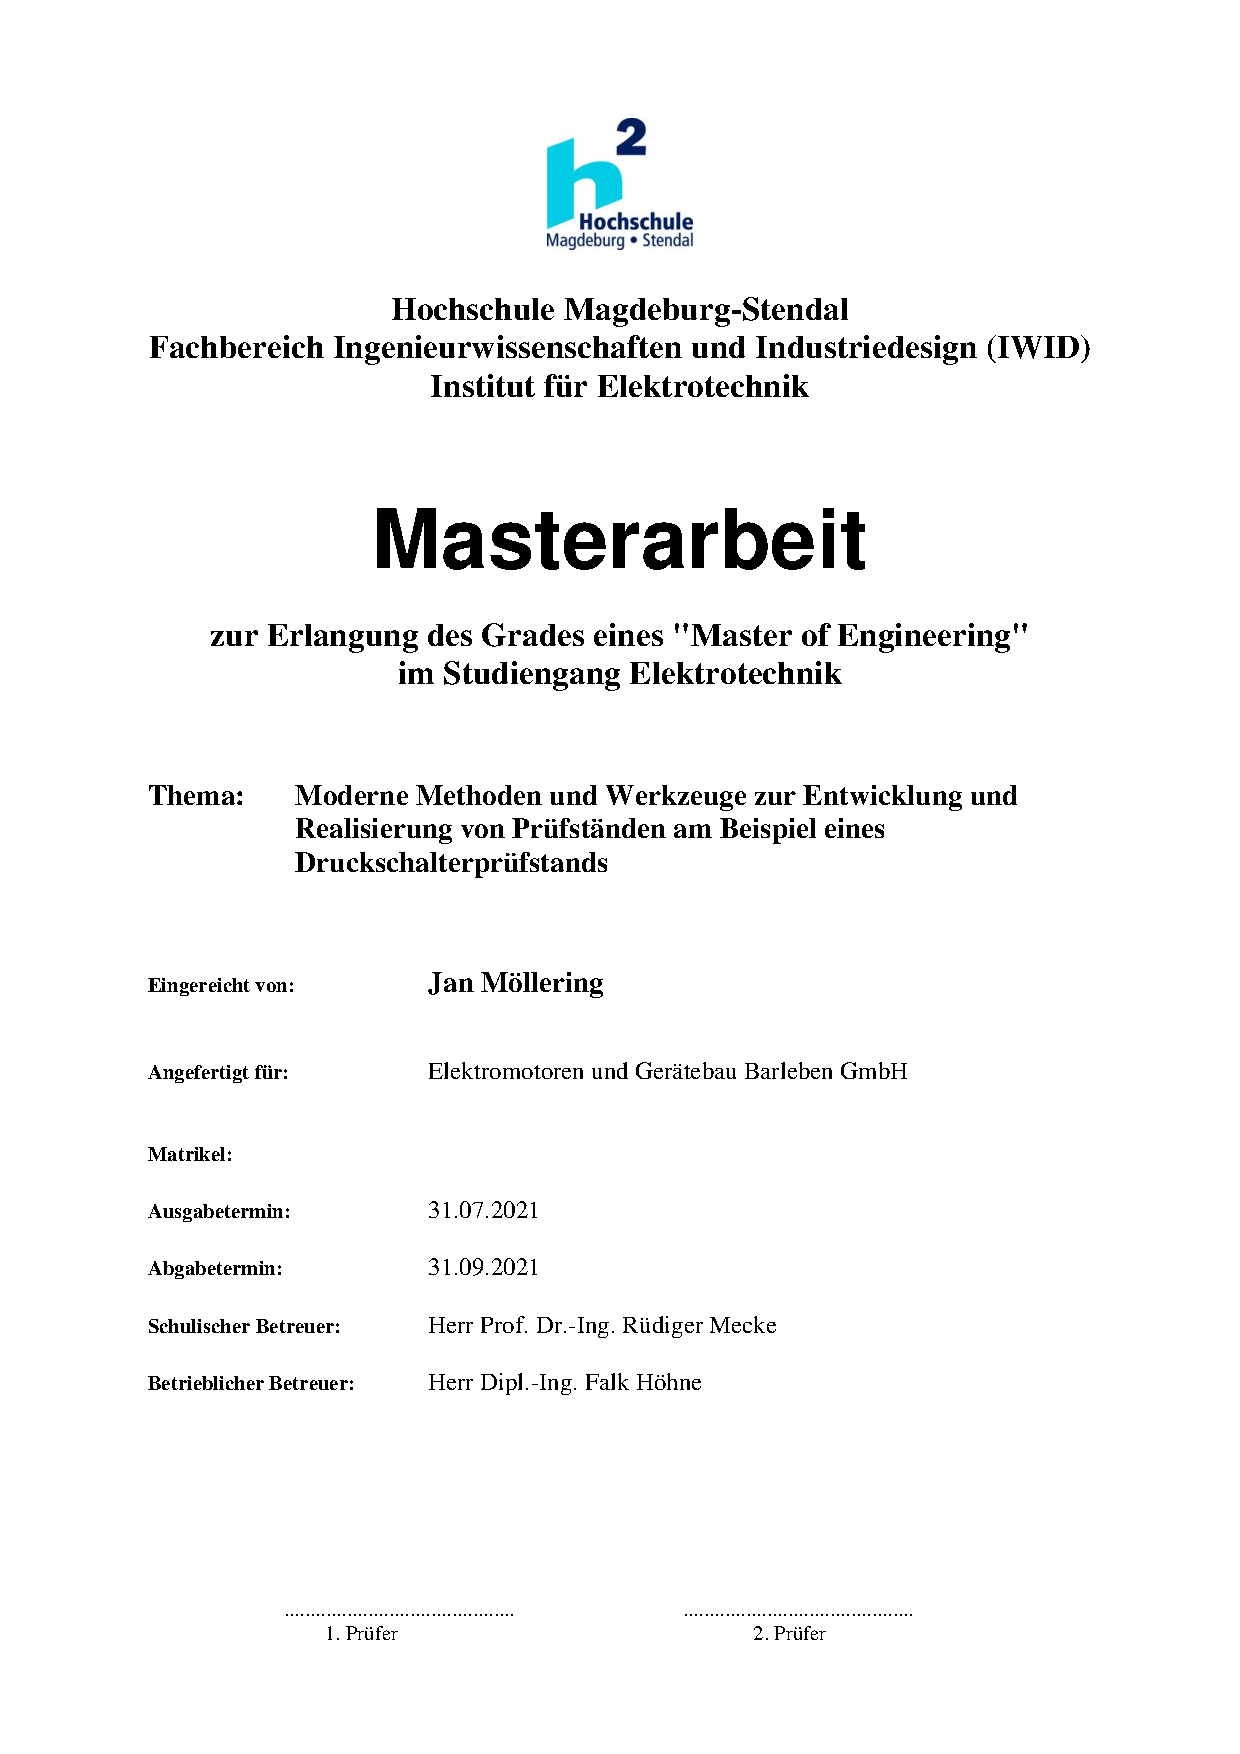
\includepdf{../Musterdeckblatt_Master.pdf}

\chapter*{Eidesstattliche Erklärung}
\thispagestyle{empty}
Hiermit erkläre ich, dass ich die vorliegende Arbeit eigenständig und ohne fremde Hilfe angefertigt habe. Textpassagen, die wörtlich oder dem Sinn nach auf Publikationen oder Vorträgen anderer Autoren beruhen, sind als solche kenntlich gemacht.
\\
\noindent
Die Arbeit wurde bisher keiner anderen Prüfungsbehörde vorgelegt und auch noch nicht veröffentlicht.

\vspace{4cm}

\hspace{2cm} Ort, Datum \hfill Unterschrift \hspace{2cm}

\chapter*{Abstract}
\thispagestyle{empty}
Diese Arbeit beschäftigt sich mit der Konzeptionierung und Realisierung eines Einzelprüfstands für Buchholz- und Gasrelais. Es wird die Elektronik und die Software entwickelt und erklärt. Teile des fertigen Prüfstands werden auf ihre Funktionen überprüft und die Testergebnisse vorgestellt.
\\
\\
\\
\\
\\
This Thesis is about the development of a concept of a test bench and its implementation. The test bench is for buchholz- and gasrelays. The electronics and software are developed and explained. Parts of the finished test bench are being tested. The results will be presented.

\setcounter{tocdepth}{2}
\tableofcontents
\thispagestyle{empty}
\newpage
\pagenumbering{Roman}
\addtocontents{toc}{\protect\thispagestyle{empty}}


\addcontentsline{toc}{chapter}{Tabellenverzeichnis}
\listoftables
\newpage

\addcontentsline{toc}{chapter}{Abbildungsverzeichnis}
\listoffigures

\addcontentsline{toc}{chapter}{Abkürzungsverzeichnis}
\chapter*{Abkürzungsverzeichnis}
\begin{acronym}[slmtA]
	\acro{GmbH}{Gemeinschaft mit beschränkter Haftung}
	\acro{USD}{United States Dollar}
	\acro{CSV}{Comma Seperated Values}
	\acro{PDF}{Portable Document Format}
	\acro{USB}{Universal Serial Bus}
	\acro{I2C}{Inter-Intergrated Circuit}
	\acro{UART}{Universal Asynchronous Receiver/Transmitter}
	\acro{HDMI}{High-Definition Multimedia Interface}
	\acro{IPC}{Inter Process Communication}
	\acro{DOM}{Document Object Model}
	\acro{LED}{Light Emmitting Diode}
	\acro{ADC}{Analog-to-Digital Converter}
	\acro{RTOS}{Real Time Operating System}
	\acro{OS}{Operating System}
	\acro{API}{Application Programming Interface}
	\acro{HTML}{Hypertext Markup Language}
	\acro{CSS}{Cascading Style Sheets}
	\acro{SCL}{System Clock}
	\acro{SDA}{System Data}
	\acro{JSON}{JavaScript Object Notation}
	\acro{XML}{Extensible Markup Language}
	\acro{SAR}{Successive Approximation Register}
	\acro{DAC}{Digital-to-Analog Converter}
	\acro{Mio}{Millionen}
	\acro{FiFo}{First in First out}
\end{acronym}
\newpage

\chapter{Motivation und Aufgabenstellung}
\pagenumbering{arabic}
\setcounter{page}{1}
\section{Motivation}
Die Nutzung von elektrischer Energie hat in der Menscheitsgeschichte
zu einem neuen Zeitalter geführt. Es hat zu einem riesigen Wohlstand-
und Fortschrittswachstum beigetragen. Heutzutage sind wir so sehr auf
die Nutzung von elektrischer Energie angewiesen, dass es nur noch schwer
aus dem normalen Leben wegzudenken ist. Im privaten wie im öffentlichen und
gewerblichen Bereich ist die Versorgung mit elektrischer Energie systemrelevant.
Dementsprechend wichtig ist das Verteilnetz der Netzbetreiber. Es ist äußerst wichtig,
dass es verlässlich funktioniert.
\\
Eines der wichtigsten und teuersten Bestandteile des Stromnetzes ist der Transformator.
Um eine hohe Verlässlichkeit zu gewährleisten, ist es deshalb sehr wichtig,
dass Fehlbetrieb und Fehlerfälle im Transformator frühzeitig erkannt werden können.
Bei größeren Fehlern, muss der Transformator vom Netz getrennt werden,
um eine Zerstörung zu vermeiden. Für diesen Zweck stellt Elektromotoren und Gerätebau Barleben GmbH
diverse Schutzgeräte für Transformatoren her.
\\
Um die Schutzfunktion zu gewährleisten, wird jedes Schutzgerät einer
Komplettprüfung unterzogen. Für eine aussagekräftige und verlässliche Prüfung
werden spezielle Prüfstände und Prüfgeräte benötigt. Die Entwicklung und Realisierung
solcher Prüfstände kann mit Hilfe von vielen unterschiedlichen Werkzeugen und Methoden
erfolgen. In den letzten Jahren sind besonders im Informationstechnik-Bereich große Fortschritte
erziehlt worden, wodurch sich neue Methoden und Werkzeuge für die Entwicklung und Realisierung
von Prüfständen ergeben haben.
\\
Am Beispiel eines Druckschalterprüfgeräts soll der Entwicklungs- und Realisierungsprozess mit Hilfe
von modernen Methoden und Werkzeugen erläutert werden. Für Personen ohne Vorwissen sollen die
unterschiedlichen zentralen Aufgabenfelder der Prüfstandsentwicklung und - realisierung vorgestellt werden.
Sie sollen einen Einblick und ein Verständnis von der Funktionsweise der Methoden und Werkzeuge und deren
Anwendung bekommen. Für Personen mit Vorwissen soll ein alternativer Lösungsweg beschrieben werden,
damit sie ihren Wissenshorizont erweitern können und einen anderen Blickwinkel auf die Thematik erlangen.

\section{Prüfstände}
Prüfstände dienen der reproduzierbaren Prüfung von technischen Gegenständen auf seine Eigenschaften.
Bestandteile eines Prüfstands ist die Aufnahme des Prüflings, die Sensorik zum Erfassen der zu prüfenden Eigenschafen,
die Aktorik zum Erzeugen der Prüfbedingungen, die Steuerung des Prüfstands
und die Datenverarbeitung der generierten Messwerte. Es wird zwischen Entwicklungs- und EoL
(\textit{englisch: End of Line}) Prüfständen unterschieden.
\\
\textbf{Entwicklungsprüfstände} dienen der Entwicklung neuer Produkte oder der Prüfung von Protoypen.
Sie verlangen meist eine höhere Spannweite in den einzustellenden Prüfbedingungen und eine genauere
Anzeige der Messwerte. Die Prüflinge müssen zum Teil unter Extrembedingungen oder über sehr lange Zeiträume
getestet werden.
\\
\textbf{EoL-Prüfstände} dienen der Qualitätskontrolle der Produktion. Sie prüfen am Ende des Produktionspozesses,
ob das gefertigte Produkt alle relevanten Eigenschaften und Funktionen in einem ausreichenden Maß besitzt.
Im Gegensatz zu den Entwicklungsprüfständen sind die Prüfbedingungen von EoL-Prüfständen meist fest vorgegeben
und benötigen keinen so großen Einstellbereich. Auch die Anzeige der Messwerte sollte sich auf das Wesentliche
beschrenken, damit die relevanten Informationen schnell und sicher dem Prüfstand entnommen werden können.

\section{Detaillierte Anforderungen an das Prüfgerät}
Als Beispiel, an dem die Methoden und Werkzeuge zur Prüfstandsentwicklung vorgestellt werden,
dient ein Druckschalterprüfgerät. Dieses Druckschalterprüfgerät soll als EoL-Prüfstand Druckschalter
testen, welche in Schutzgeräten für Hermetiktransformatoren eingebaut sind. Für ein besseres Verständnis
soll an dieser Stelle auf das Schutzgerät an sich und auf die Anforderungen des Prüfgeräts eingegangen werden.

\subsection{Schutzgerät CF38 mit Druckschalter}
Das Gasrelais CF38 mit Druckschalter wurde für hermetisch abgeschlossene Transformatoren entwickelt.
Hermektik-Transformatoren wurden entwickelt, weil Sauerstoff in der Umgebungsluft einen großen Einfluss
auf den Alterungsprozess und damit auf die Lebensdauer eines Transformators hat. Durch den hermetischen
Abschluss wird ein Luftaustausch mit der Umgebungsluft unterbunden und damit die Lebensdauer erhöht.
Einer der großen Nachteile gegenüber herkömmlichen Transformatoren ist,
dass es schwieriger ist bei Temperaturschwankungen mit sich ausdehnendem Öl umzugehen.
Es kann ein hoher Druck im Transformator entstehen. Um Beschädigungen des Transformators
zu verhindern, schaltet der Druckschalter im CF38 Gasrelais bei einem bestimmten Grenzwert.
Am Ende des Produktionsprozesses muss überprüft werden, ob der Druckschalter innerhalb eines
Toleranzbereichs des angegebenen Grenzwerts schaltet.
Für die Überprüfung wird ein Druckschalterprüfgerät entwickelt. Dafür haben sich bestimmte Anforderungen ergeben.

\subsection{Anforderungen}
Das Prüfgerät soll Druckschalter überprüfen, die im CF38 Gasrelais eingebaut sind.
Der Schaltpunkt des Druckschalters kann bis zu 1\,bar betragen. Die Messmittelfähigkeit
soll anschließend überprüft und verifiziert werden.

\subsubsection{Durchzuführende Prüfungen}
Es sollen mindestens zwei Druckschalter gleichzeitig geprüft werden. Dabei sollen der Einschaltpunkt
und der Ausschaltpunkt von Schließer- und Öffner-Kontakten bestimmt werden.

\subsubsection{Hardwareentwicklung}
Für das Prüfgerät soll eine Platine entworfen werden. Kernfunktion dieser Platine ist es eine hochpräzise
Strommessung im Bereich 0-20\,mA zu ermöglichen. Ein geeignetes Schaltungsdesign ist zu wählen.
\\
Es muss außerdem im Hinblick auf die Messungen und der grafischen Oberfläche ein geeigneter Mikrocontroller
oder Entwicklungsboard ausgewählt werden.

\subsubsection{Entwicklung einer grafischen Anzeige}
Auf einem Display sollen die Messwerte in geeigneter Form angezeigt werden.
Es ist auf eine übersichtliche Darstellung zu achten, bei der nur die benötigten
Informationen angezeigt werden. Die Bedienung erfolgt über einen Drehknopf.
\\
Bei dem Display soll es sich um ein 4.3'' oder 5'' LCD-Display handeln.

\subsubsection{Mobilität durch integrierte Spannungsversorgung}
Das Prügerät soll mobil ohne externe Spannungsversorgung funktionieren.
Es soll sich um ein Handgerät handeln. Dafür muss eine interne Spannungsquelle ausgewählt
und die dazugehörige Elektronik für die Platine entwickelt werden.

\subsubsection{Datenverarbeitung und -speicherung}
Es soll die Möglichkeit geben, die Messwerte an eine zentrale Datenverarbeitungseinheit zu senden.
Die Verbindung kann dabei mit Kabel oder kabellos erfolgen.
\\
\\
Die Messwerte sollen zentral in einem geeigneten Dateiformat gespeichert werden.
Aus den Messwerten soll auch ein Protokoll erstellt werden, welches auch vom Messgerät
ausgedruckt werden kann. Von unterschiedlichen Computern soll über das firmeninterne Netzwerk
auf die gespeicherten Daten zugegriffen werden können.

\subsubsection{}



\section{Aufgabenstellung}

\textbf{Die Teilaufgaben umfassen:}

\begin{itemize}
	\item Einarbeitung in die ...
	\item Entwicklung der Elektronik für das Prüfgerät
	\begin{itemize}
		\item Unterpunkt 1
		\item Unterpunkt 2
		\item Messen von Stromwerten im \(\mu\)A Bereich
	\end{itemize}
	\item Entwicklung und Programmierung der Software für das Prüfgerät
	\begin{itemize}
		\item Steuerung des Prüfgeräts
		\item Darstellung, Speicherung und Auswertung der Messwerte
		\item Realisierung einer grafischen Oberfläche
	\end{itemize}
	\item Auswahl aller benötigten Komponenten
	\item Aufbau eines funktionsfähigen Prototyps des Prüfgeräts
	\item Erprobung und Testung von Teilkomponenten
\end{itemize}

\chapter{Messtechnik}
\section{Grundlagen Sensoren}
Hier stehen die Grundlagen für Sensoren

\section{Analog Digital Wandler}

\section{SAR ADC}

\section{Delta-Sigma ADC}

\section{Schaltungsdesign Strommessung}

\chapter{Mikrocontroller-Programmierung}
\section{Grundlagen der Mikrocontroller-Programmierung}

\section{Echtzeitbetriebssysteme}

\section{Schrittketten-Programmierung}

\section{Steuerung-Programmierung}

\chapter{Kommunikation}
\section{USB}

\section{Bus Systeme}

\subsection{RS232}

\subsection{RS485}

\subsection{CAN}

\subsection{Ethernet}

\subsection{I2C}

\subsection{SPI}

\section{Protokolle}

\subsection{Modbus}

\subsection{Profibus}

\subsection{TCP/IP}

\subsection{MQTT}

\chapter{Grafische Benutzeroberfläche}
\section{Grundlagen}

\subsection{Hardware}

\subsection{Model-View-Presenter Struktur}

\section{Material Design}

\subsection{Farbsystem}

\subsection{Layoutsystem}

\subsection{Typografiesystem}

\subsection{Dark Theme}

\section{Framework}

\subsection{Embedded wizard}

\subsection{TouchGFX}

\subsection{LVGL}

\subsection{Qt for MCU}

\subsection{Electron und React}

\chapter{Datenverarbeitung}
\section{JSON Datenformat}

\section{Serielle Schnittstelle mit Python}

\section{Dokumentengenerierung}

\subsection{Word}

\subsection{PDF}

\subsection{Excel}

\subsection{CSV}

\chapter{Messsystemanalyse}
\section{Genauigkeit}

\section{Stabilität}

\section{Präzision}

\chapter{Zusammenfassung und Ausblick}
\section{Zusammenfassung}

\section{Ausblick}

\printbibliography

\appendix



\end{document}